\documentclass[a4paper,12pt]{article}
\usepackage{a4wide}
\usepackage{tikz}
\usetikzlibrary{calc}
\usepackage{hyperref}
\usepackage{pdflscape}
\usepackage{../static/bytefield} % relative to tmp

\usepackage[ngerman]{babel}

\newlength{\maxheight}
\setlength{\maxheight}{\heightof{W}}
\newcommand{\baselinealign}[1]{ %
	\centering
	\raisebox{0pt}[\maxheight][0pt]{ #1} %
}

\newcommand\Tstrut{\rule{0pt}{2.6ex}}       % "top" strut

\definecolor{grau}{gray}{.5}

\begin{document}
\pagestyle{empty}
\setlength{\parindent}{0em}
\section*{\noindent Multicycle Control Unit }
Ihre Aufgabe ist es, das Verhalten einer Entity  namens "`MC\_CU"' zu programmieren. Die Entity ist in der angeh\"angten Datei "`MC\_CU.vhdl"' mit folgenden Eigenschaften deklariert:

\begin{itemize}
	\item Eingang: CLK vom Typ std\_logic
	\item Eingang: Opcode vom Typ std\_logic\_vector mit einer L\"ange von 6
	\item Eingang: Funct vom Typ std\_logic\_vector mit einer L\"ange von 6
	\item Eingang: Zero vom Typ std\_logic

	\item Ausgang: PCSrc vom Typ std\_logic\_vector mit einer L\"ange von 2
	\item Ausgang: ALUControl vom Typ std\_logic\_vector mit einer L\"ange von 3
	\item Ausgang: ALUSrcB vom Typ std\_logic\_vector mit einer L\"ange von 2
	\item Ausg\"ange: IRWrite, MemWrite, IorD, PCWrite, ALUSrcA, RegWrite, MemtoReg, RegDst vom Typ std\_logic

\end{itemize}

\begin{center}
\begin{tikzpicture}
\draw node [draw,rectangle, minimum height=72mm, minimum width=35mm,rounded corners=2mm,thick](entity){};

\draw[->] ($ (entity.west)+(-10mm,21.6mm)$) -- ($ (entity.west) + (0mm,21.6mm)$);
\draw[anchor=east] node at ($ (entity.west)+(-9mm,21.6mm)$){ CLK };

\draw[->] ($ (entity.west)+(-10mm,7.2mm)$) -- ($ (entity.west) + (0mm,7.2mm)$);
\draw[anchor=east] node at ($ (entity.west)+(-9mm,7.2mm)$){ Opcode };

\draw[->] ($ (entity.west)+(-10mm,-7.2mm)$) -- ($ (entity.west) + (0mm,-7.2mm)$);
\draw[anchor=east] node at ($ (entity.west)+(-9mm,-7.2mm)$){ Funct };

\draw[->] ($ (entity.west)+(-10mm,-21.6mm)$) -- ($ (entity.west) + (0mm,-21.6mm)$);
\draw[anchor=east] node at ($ (entity.west)+(-9mm,-21.6mm)$){ Zero };


\draw[->] ($ (entity.east) + (0mm,30.0mm)$) -- ($ (entity.east) + (10mm,30.0mm)$);
\draw[anchor=west] node at ($ (entity.east) + (9mm,30.0mm)$){ IRWrite };

\draw[->] ($ (entity.east) + (0mm,24.0mm)$) -- ($ (entity.east) + (10mm,24.0mm)$);
\draw[anchor=west] node at ($ (entity.east) + (9mm,24.0mm)$){ MemWrite };

\draw[->] ($ (entity.east) + (0mm,18.0mm)$) -- ($ (entity.east) + (10mm,18.0mm)$);
\draw[anchor=west] node at ($ (entity.east) + (9mm,18.0mm)$){ IorD };

\draw[->] ($ (entity.east) + (0mm,12.0mm)$) -- ($ (entity.east) + (10mm,12.0mm)$);
\draw[anchor=west] node at ($ (entity.east) + (9mm,12.0mm)$){ PCWrite };

\draw[->] ($ (entity.east) + (0mm,6.0mm)$) -- ($ (entity.east) + (10mm,6.0mm)$);
\draw[anchor=west] node at ($ (entity.east) + (9mm,6.0mm)$){ PCSrc };

\draw[->] ($ (entity.east) + (0mm,0.0mm)$) -- ($ (entity.east) + (10mm,0.0mm)$);
\draw[anchor=west] node at ($ (entity.east) + (9mm,0.0mm)$){ ALUControl };

\draw[->] ($ (entity.east) + (0mm,-6.0mm)$) -- ($ (entity.east) + (10mm,-6.0mm)$);
\draw[anchor=west] node at ($ (entity.east) + (9mm,-6.0mm)$){ ALUSrcB };

\draw[->] ($ (entity.east) + (0mm,-12.0mm)$) -- ($ (entity.east) + (10mm,-12.0mm)$);
\draw[anchor=west] node at ($ (entity.east) + (9mm,-12.0mm)$){ ALUSrcA };

\draw[->] ($ (entity.east) + (0mm,-18.0mm)$) -- ($ (entity.east) + (10mm,-18.0mm)$);
\draw[anchor=west] node at ($ (entity.east) + (9mm,-18.0mm)$){ RegWrite };

\draw[->] ($ (entity.east) + (0mm,-24.0mm)$) -- ($ (entity.east) + (10mm,-24.0mm)$);
\draw[anchor=west] node at ($ (entity.east) + (9mm,-24.0mm)$){ MemtoReg };

\draw[->] ($ (entity.east) + (0mm,-30.0mm)$) -- ($ (entity.east) + (10mm,-30.0mm)$);
\draw[anchor=west] node at ($ (entity.east) + (9mm,-30.0mm)$){ RegDst };


\draw node at ($ (entity) - (0,0mm)$){ MC\_CU };

\end{tikzpicture}
\end{center}

Ver\"andern sie die Datei "`MC\_CU.vhdl"' nicht!\\

Sie m\"ussen folgende verschiedene Instruktions-Typen implementieren:

{{selected_instruction_type_text}}


Vor der Ausf\"uhrung einer Instruktion muss diese zuerst aufgerufen (fetch) und decodiert (decode) werden. Dieser Vorgang ben\"otigt 2 Taktzyklen.  W\"ahrend des Fetch-Taktzyklus wird die Instruktion von dem aktuellen Befehlsz\"ahler (PC-Wert) gelesen und in das Instruktionsregister gespeichert. Au"serdem wird in diesem Zyklus das PC Register mittels der ALU um 4 erh\"oht. Im zweiten Taktzyklus wird die Instruktion im Steuerwerk (control unit) decodiert. {{beq_bne_decode_addition}} \\

Die `MC\_CU"' Entity soll den Multicycle Prozessor, welcher in Abbildung~1 dargestellt ist, so steuern, dass folgende Instruktionen ausgef\"uhrt werden k\"onnen:

\begin{table}[h!]
\centering
    \begin{tabular}{|c|c|c|c|c|} \hline \Tstrut
		instruction & opcode  & funct & type   \\ \hline \Tstrut
		{{selected_instruction_table_text}}
    \hline
    \end{tabular}
\end{table}

{{first_instruction_text}} \\

{{second_instruction_text}} \\

\begin{table}[h!]
\centering
    \begin{tabular}{|c|c|} \hline \Tstrut
		ALUControl & Function   \\ \hline \Tstrut
		{{ALUControl_table}}
    \hline
    \end{tabular}
    \caption{ALUControls}
    \label{tab:ALUControls}
\end{table}

Um ein besseres Verst\"andnis f\"ur die Steuersignale zu erhalten, sei hier eine Beschreibung aller Signale gegeben. Verwenden Sie Abbildung~1 um zu verstehen, wie die Steuersignale die Datenpfade steuern.

\begin{itemize}

\item{IRWrite: Wenn dieses Signal auf '1' gesetzt ist, dann wird die aus dem Instruktionsspeicher gelesene Instruktion bei steigender Tanktflanke in das Instruktionsregister geschrieben.}

\item{MemWrite: Wenn dieses Signal auf '1' gesetzt ist, dann schreibt der Datenspeicher die Eingangsdaten "`Write data"' bei steigender Taktflanke an die Zieladresse "`Address"'.}

\item{IorD: Bestimmt, ob die Eingangsadresse "`Address"' des Datenspeichers durch das PC Register oder das Result Register der ALU ausgew\"ahlt wird.}

\item{PCWrite: Wenn dieses Signal auf '1' gesetzt ist, dann wird das PC Register bei steigender Taktflanke beschrieben.}

\item{PCSrc: Bestimmt, ob der neue PC-Wert direkt von der ALU, dem ALU Result Register oder der Sprungadresse festgelegt wird.}

\item{ALUControl: W\"ahlt jene ALU Operation aus, welche die ALU auf ihre zwei Eingangswerte anwendet. Die Steuersignale f\"ur die verf\"ugbaren Operationen sind in Tabelle~1 gelistet.}

\item{ALUSrcB:  Bestimmt, ob die ALU einen Wert von dem Register Ausgang "`Read data 2"', von einem konstanten Wert 4, von dem vorzeichenerweiterten IMM-Wert der Instruktion oder von dem vorzeichenerweiterten und um 2 Bit nach links geschobenen IMM-Wert der Instruktion erh\"alt.}

\item{ALUSrcA: Bestimmt, ob die ALU einen Wert von dem Register Ausgang "`Read data 1"' oder von dem PC Register erh\"alt.}

\item{RegWrite: Wenn dieses Signal auf '1' gesetzt ist, dann schreibt das Register die Daten "`Write data"' bei steigender Taktflanke in das durch "`Write register"' adressierte Register.}

\item{MemtoReg: Bestimmt, ob die in das Register zu schreibenden Daten "`Write data"' entweder vom Ausgang des Datenspeichers "`Read I/D"' oder dem ALU Result Register kommen.}

\item{RegDst: Bestimmt, ob die Position des zu beschreibenden Registers "`Write Register"' entweder von den Bits 20 -- 16 oder 15 -- 11 der Instruktion definiert wird. In anderen Worten entscheidet dieses Steuersignal, ob das zu beschreibende Register durch rt oder rd festgelegt wird.}

\end{itemize}

\"Uberlegen Sie sich, welche Aktion jeder Teil des Prozessors f\"ur die Funktion der jeweiligen Instruktionen erf\"ullen muss und setzen Sie die Steuersignale entsprechend. Programmieren Sie dieses Verhalten in der angeh\"angten Datei "`MC\_CU\_beh.vhdl"'.\\

Um Ihre L\"osung abzugeben, senden Sie ein E-Mail mit dem Betreff "`Result Task {{ TASKNR }}"' und Ihrer Datei "``MC\_CU\_beh.vhdl"'  an {{ SUBMISSIONEMAIL }}.

\vspace{0.7cm}
Viel Erfolg und m\"oge die Macht mit Ihnen sein.


\begin{landscape}
\begin{figure}[!h]
\vspace{-1cm}
\hspace{-1.8cm}
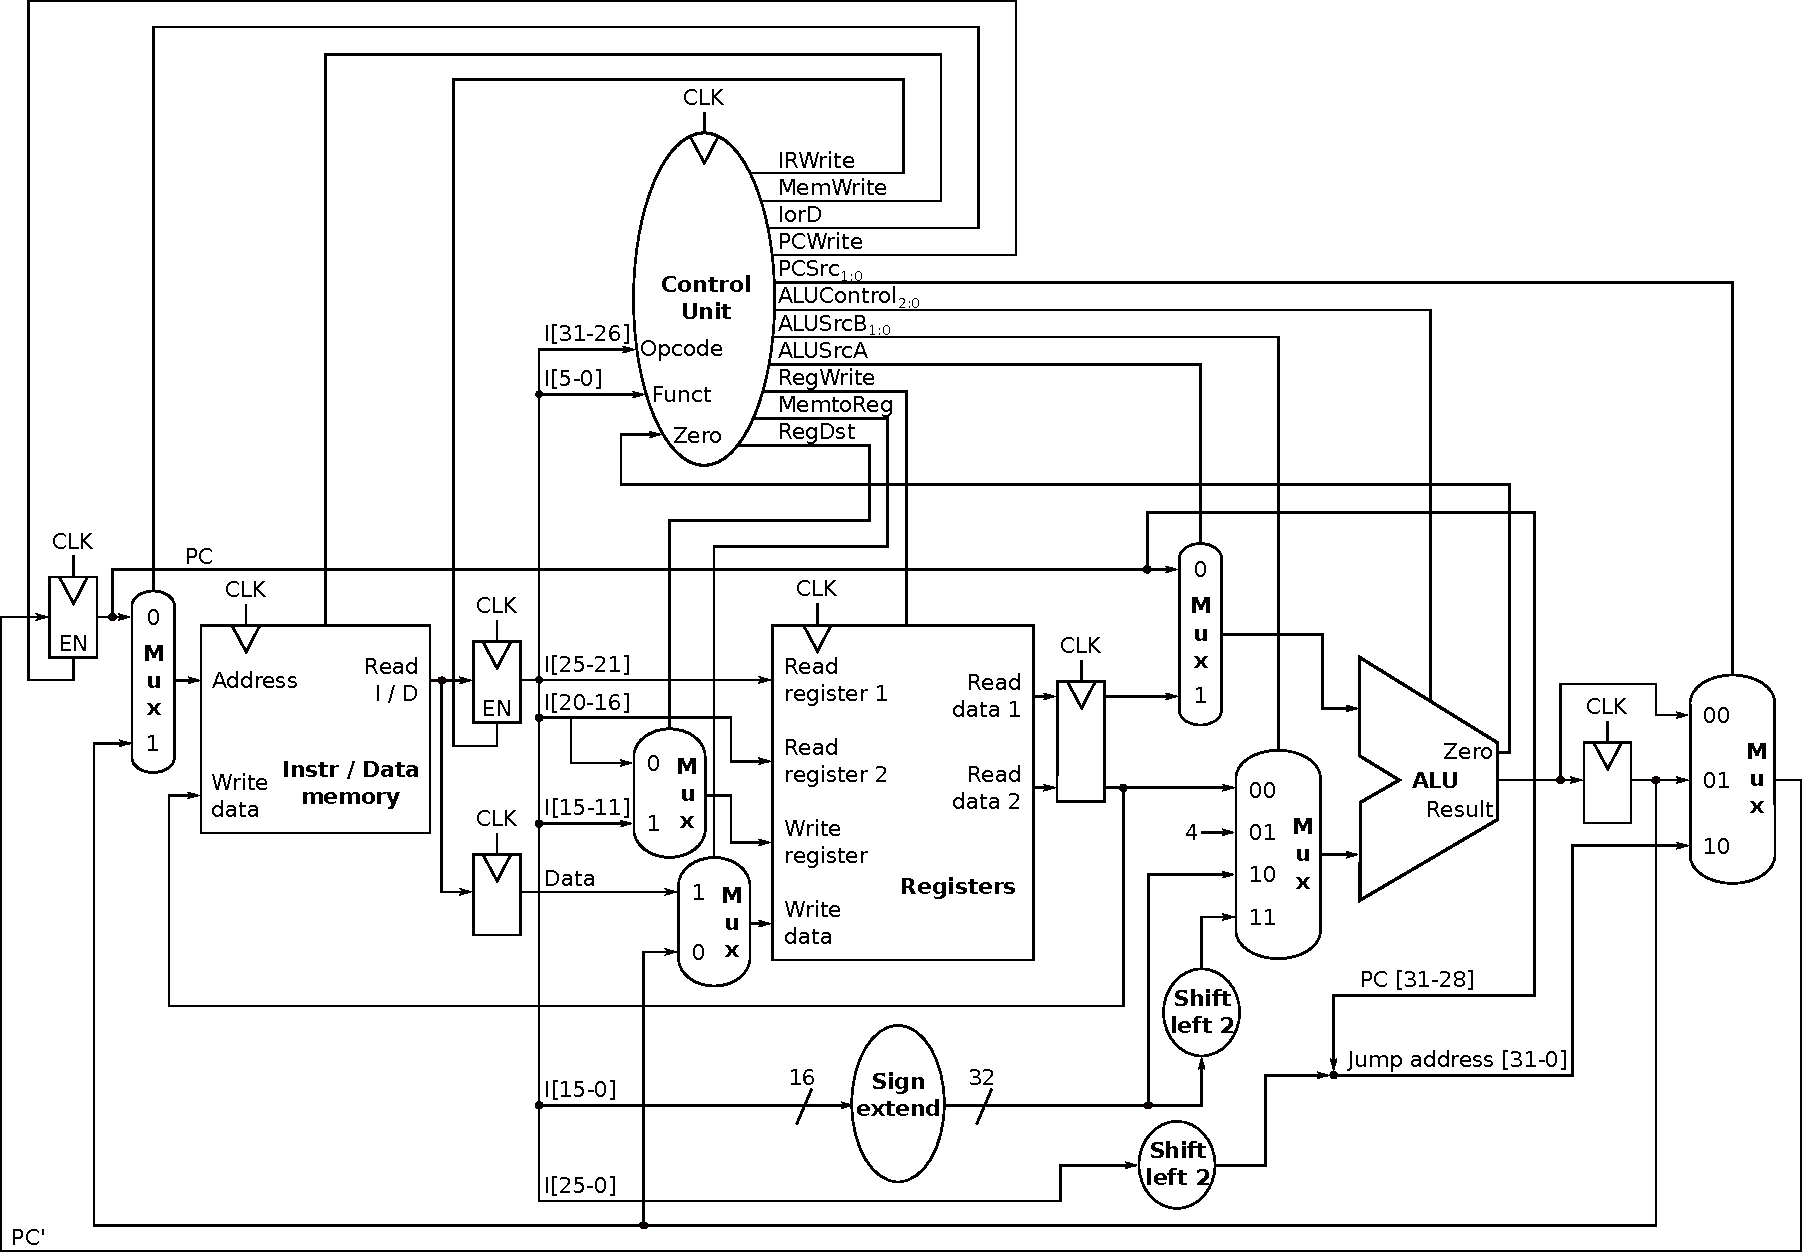
\includegraphics[width=25.5cm]{../static/Multicycle_Processor_V_1_3} % relative to tmp
\caption{Multicycle processor}
\label{fig:MulticycleProcessor}
\end{figure}
\end{landscape}

\end{document}
